\subsection{CalvinFS}
CalvinFS \cite{DBLP:conf/fast/ThomsonA15} is an experimental distributed file-system created with the goal of exploring the performance and scalability implications of metadata storage in a (distributed) database system.
The distributed database is CalvinDB \cite{DBLP:conf/sigmod/ThomsonDWRSA12}, created by same of the same authors, a share-nothing distributed database with support for high-performance distributed transactions.

\subsubsection{Architecture}
\begin{figure}[h]
\caption{CalvinFS architecture diagram}
\label{fig:calvin-block-diagram}
\centering
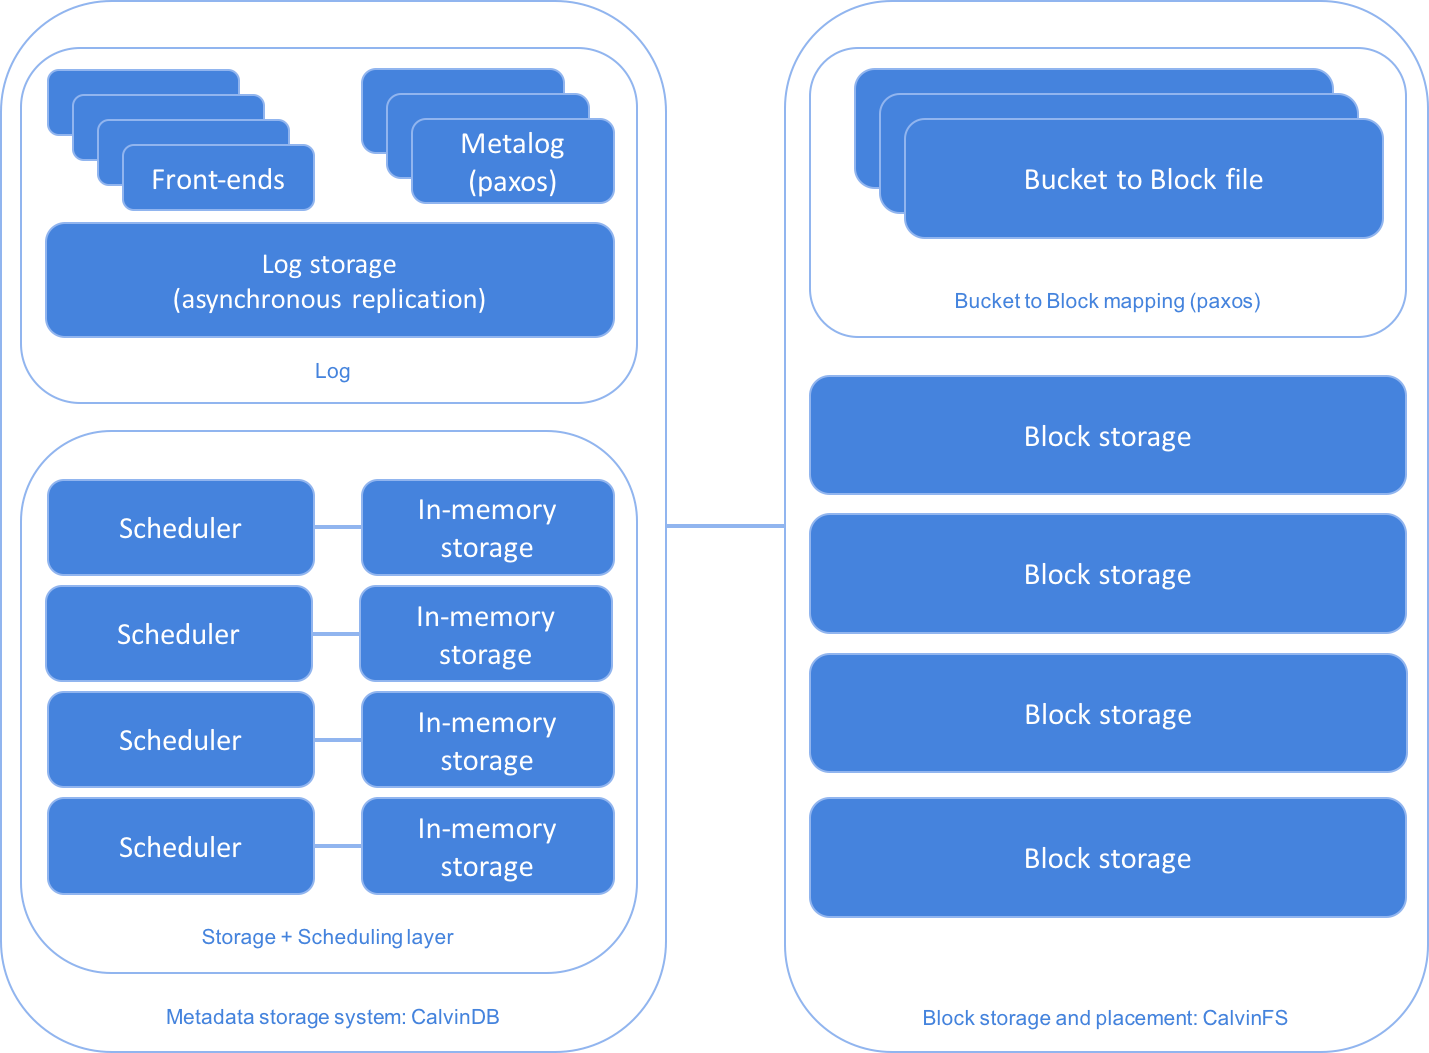
\includegraphics[width=1.0\textwidth]{images/calvin-block-diagram.png}
\end{figure}


Much like previously discussed distributed file-systems, the system is designed around two components, as shown in Figure \ref{fig:calvin-block-diagram}:
\begin{itemize}
    \item a \emph{metadata store} which maintains information about file-system hierarchy, permissions, file-to-block mappings and replica locations, and
    \item a \emph{block store} which stores physical data on disk in blocks and provides primitives to read and write such blocks.
\end{itemize}

\paragraph{Metadata store} The \emph{metadata store} is CalvinDB, extended with a number of filesystem-specific operations.
CalvinDB is itself divided into three components: \begin{inparaenum}[i)]
    \item a \emph{log} which maintains an ordered list of transactions with parameters,
    \item a \emph{storage} layer which stores database data and provides local transaction semantics, and
    \item a \emph{scheduling} layer which performs local execution of transactions.
\end{inparaenum}
Each of these components is exposed to others through a standard interface and can therefore be replaced independently.

In CalvinDB, the \textbf{log} maintains a complete and ordered list of transactions and transaction parameters, such that, by replaying all transactions from this log the database can be reconstructed.
The log is completely distributed and is divided in two logical components: front-end servers and the metalog.
Front-end servers accept transaction requests from clients and batch them before writing such batches in the distributed storage.
Once the batch is safely stored (and replicated) in the storage, the system generates a unique ID in the batch and writes it in the metalog.
The metalog is a ordered sequence of unique batch IDs maintained by a set of servers running a Paxos consensus protocol for consistency.
In order to ``replay'' transactions, the system traverses the metalog extracting the unique IDs and executes the transaction batches in that order.

The \textbf{storage layer} organizes the storage of database data.
As all the other components, the storage layer is an interface and any implementation fulfills the following criterias: 
\begin{inparaenum}[i)]
    \item provides read and write primitives that execute on the node,
    \item provides a placement manager that, for every request, provides a storage node where the operation can be executed and
    \item allows the definition of custom transactions that include both read/write primitives and other deterministic application-specific logic.
\end{inparaenum}
The ability to define custom transactions is particularly powerful in the context of a distributed file-system as it provides the opportunity to define more high-level operations such as \texttt{CreateFile(path)} that will be serialized in the log along with all their arguments (\texttt{path} in this case).
The implementation used in CalvinFS provides a in-memory key-value store which supports versioning of keys and uses consistent hashing of keys to determine placement of values.

The \textbf{scheduler} drives local query execution and one process is therefore executed alongside every storage layer node.
Unlike most other database systems which employ a pessimistic locking scheme and wait for locks when they are acquired by another transaction, the scheduler in CalvinDB uses a protocol called deterministic locking that analyzes the entire transaction, determines the read/write set and executes it only when it is safe to do so without additional checks.
The actual execution is performed by the storage node when the scheduler forwards the transaction to it.
The absence of a distributed commit protocol, usually required by other database systems in this scenario, greatly increases scalability and reduces latency.
It, however, limits the type of transactions that can be executed to those for which the read/write set can be determined statically (without executing the query itself).
Given that some operations, such as recursive change of permissions, require transactions for which the read/write set cannot be statically determined, a system called OLLP (Optimistic Lock Location Prediction) is used to estimate the read write set.
The implementation of OLLP for CalvinFS executes the query without performing writes (a dry-run) and then annotates the transaction with the read/write set obtained.
If the read/write set provided by the dry-run is different from the one obtained during actual execution due to changes in the data, the new set is appended to the transaction and the transaction is restarted.

\paragraph{File-system metadata organization} CalvinFS stores file metadata as an association between a key, the full path of the object, and a value containing various fields: \begin{itemize}
    \item Type: either file or directory,
    \item Permissions: unix-like permissions for the object and all ancestors,
    \item Content (directory): a list of all files contained in the directory including subdirectories and
    \item Content (file): A mapping between byte-ranges in the file and block IDs.
\end{itemize}

Given the flat organization of files and the fact that all files store permissions for all the ancestors, changing permissions of a directory is potentially a very expensive operation as it involves changing all the descendants.
Recursive queries are also very expensive for the same reason.

\paragraph{Block store} Block storage in CalvinFS differs from the file-systems previously discussed in two significant ways: block allocation and block assignment.
Blocks in CalvinFS are completely immutable and can range from 1 byte to 10 megabytes.
Every write operation generates an entire new immutable block and appends it to the file metadata.
A background process periodically rewrites and compacts blocks in order to reduce fragmentation but blocks are otherwise completely immutable.
Each block is assigned a global ID which is stored in the metadata and, in order to be assigned to a set of machines, the block ID is hashed and the hash is used to identify a bucket.
Each bucket is assigned to a set of machine and those machine are responsible for all the files whose ID hash is in the bucket.
The mapping of machine to buckets is maintained in a Paxos replicated store and is additionally cached on all machines.

\paragraph{Geographical replication} All of the components discussed above can be executed in geographically distant data-centers and the system assigns replicas in a way that minimizes disruption during failures and network partitions.
Most operations only need a quorum of machines to acknowledge before returning to the client, therefore the latency of the overall system in the case of three geographic areas (the typical case) depends on the two areas with the lowest latency to the client (the third will eventually ack).